%%%%%%%%%%%%%%%%%%%%%%%%%%%%%%%%%%%%%%%
%%  MISCELLANEOUS SETTINGS/COMMANDS  %%
%%%%%%%%%%%%%%%%%%%%%%%%%%%%%%%%%%%%%%%


\newcommand{\balA}[1][1]{BAL$^\mathup{I}_{#1:#1}$\xspace}
\newcommand{\unbalA}[1][n]{UNBAL$^\mathup{I}_{1:#1}$\xspace}
\newcommand{\balB}[1][1]{BAL$^\mathup{II}_{#1:#1}$\xspace}
\newcommand{\unbalB}[1][n]{UNBAL$^\mathup{II}_{#1:1}$\xspace}

%% Add separator slide to the beginning of each section ==>
\AtBeginSection[]{
	\begin{frame}[standout, c]{~}
		%\vfill
		\usebeamerfont{title}%
		\textcolor{SpotColor}{\insertsectionhead}
		%\vfill
	\end{frame}%
}

%% Alternativelyy, add ``Outline'' slide to the beginning of each section ==>
%\AtBeginSection[]{
%	\begin{frame}[plain]{Outline}
%		\tableofcontents[currentsection]
%	\end{frame}
%}
%% <==

\title{Introduction of Reduced Convolutional Networks}

\subtitle{精简卷积神经网络简介}

\author[唐呈俊]{%
	唐呈俊
} % Author(s)

\institute{%
	桂林电子科技大学
} % Institution(s)

\date{%
	%\\
	%Name of the Inviting %Institution/Seminar Series
	\\[\medskipamount]
	\textmd{\today}%
}




%%%%%%%%%%%%%%%%%%%
%%  TITLE SLIDE  %%
%%%%%%%%%%%%%%%%%%%


\begin{frame}[standout]{~}

	\titlepage%

\end{frame}


\begin{frame}[standout]{Outline}

	\medskip
	\tableofcontents

\end{frame}




%%%%%%%%%%%%%%%%%
%%  MAIN PART  %%
%%%%%%%%%%%%%%%%%


\section{Preliminaries}

\begin{frame}{\titleprefix: 自学内容}
	\alert{我们假设你在学习本课程前已经了解了如下概念的内容:}
	
	\begin{description}
		\item[FC] Fully Connected Layer,全连接层
		\item[Activations] Activation Functions 激活函数
	\end{description}

	当然,基本的\alert{高等数学、线性代数、概率论}知识也是必要的。\alert{信息论}也许也会有一定的帮助。
\end{frame}

\begin{frame}{\titleprefix: 卷积层的计算}
	\begin{figure}
		\centering
		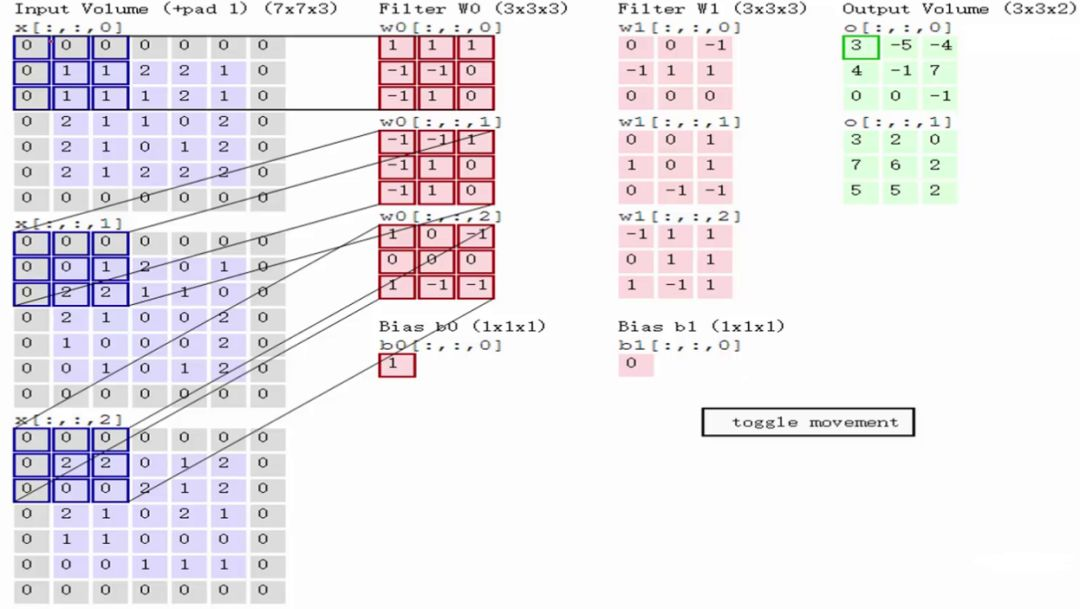
\includegraphics[width=\linewidth]{Images/conv_1}
		\caption{卷积计算过程}
		\label{fig:conv1}
	\end{figure}
	
\end{frame}

\begin{frame}{\titleprefix: 卷积层的参数}
	
	上图讲解的是一个3*3的2D卷积,那么卷积层还有什么样的参数呢:
	\begin{description}
		\item[Filter] 滤波器数量
		\item[Kernel Size] 卷积核大小
		\item[Strides] 步长
		\item[Padding] 填充
	\end{description}
	
\end{frame}

\begin{frame}{\titleprefix: 池化层}
	虽然今天没有涉及池化的优化,但卷积总是和池化分不开的:
	\begin{figure}
		\centering
		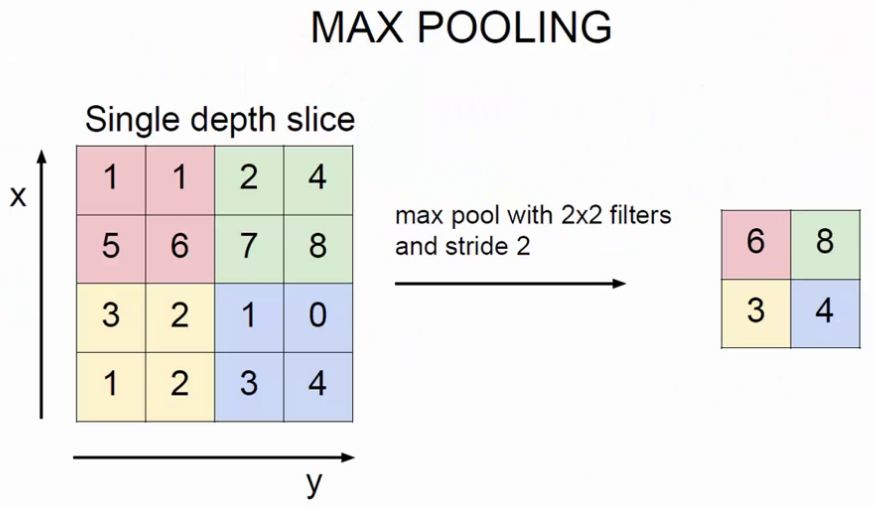
\includegraphics[width=0.7\linewidth]{Images/pool_1}
		\caption{最大池化}
		\label{fig:pool1}
	\end{figure}
\end{frame}

\section{Methodology}

\begin{frame}{\titleprefix: AlexNet}
	虽然AlexNet并非轻量化神经网络,但其中的两个方法,却是如今轻量化网络的重要基石:
	\begin{description}
		\item[Group Conv] AlexNet中,为了在两个GPU上并行训练,其将卷积分解为两个Group,从而在两个GPU上完成。
		\item[ReLU] AlexNet中,采用了ReLU激活函数,相比先前的tanh和sigmoid函数,ReLU函数的计算速度,和训练时的收敛速度都更快。
	\end{description}
\begin{figure}
	\centering
	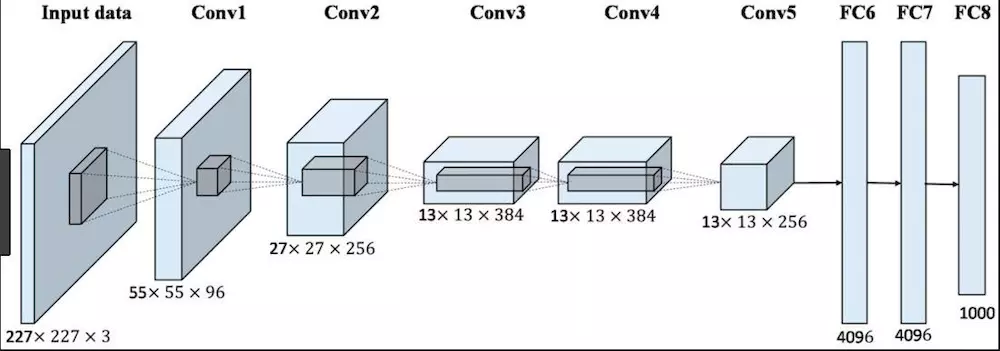
\includegraphics[width=0.7\linewidth]{Images/alexnet_1}
	\caption{AlexNet网络结构}
	\label{fig:alexnet1}
\end{figure}

\end{frame}

\begin{frame}{\titleprefix: Group Conv}
	\begin{figure}
		\centering
		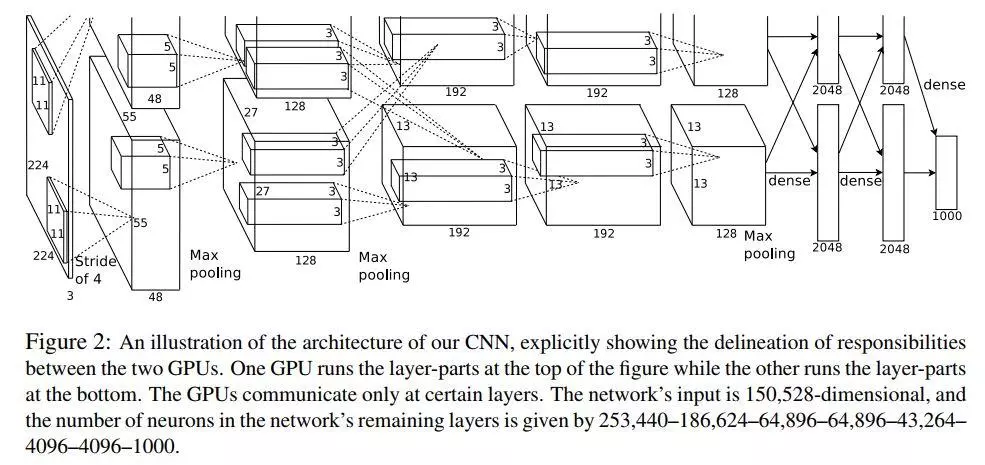
\includegraphics[width=0.9\linewidth]{Images/groupconv_1}
		\caption{AlexNet的Group Conv结构}
		\label{fig:groupconv1}
	\end{figure}
你能从中找到对应Group Conv的部分吗?
\end{frame}

\begin{frame}{\titleprefix: Depthwise Conv}
	虽然AlexNet的Group Conv的目的是将计算分配给两个GPU并行运行,但是这也同样减少了计算量。(想想看为什么)
	
	如果说将每个通道,都分到其对应的Group中,这种Group Conv的特殊情况,就将其运算量减少到了最少的情况。但这样做的代价是什么?(可以想想\alert{互信息}的概念)
\begin{figure}
	\centering
	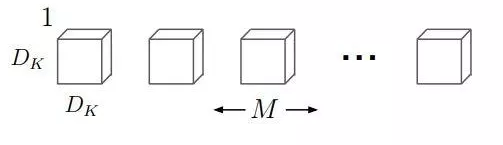
\includegraphics[width=0.7\linewidth]{Images/depthwise_1}
	\caption{Depthwise Conv,其中M是通道数,也是滤波器数}
	\label{fig:depthwise1}
\end{figure}

\end{frame}

\begin{frame}{\titleprefix: Depthwise Conv}
	\begin{figure}
		\centering
		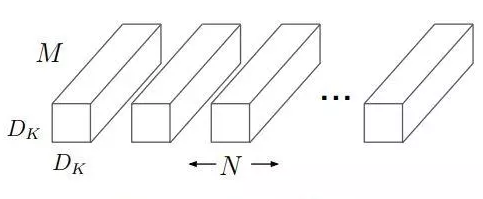
\includegraphics[width=0.5\linewidth]{Images/depthwise_2}
		\caption{标准的Conv(相对于 Depthwise Conv)}
		\label{fig:depthwise2}
	\end{figure}
	\[
\mathbf{G}_{k, l, n}=\sum_{i, j, m} \mathbf{K}_{i, j, m, n} \cdot \mathbf{F}_{k+i-1, l+j-1, m}
\text{普通卷积}
\]	
\[
\hat{\mathbf{G}}_{k, l, m}=\sum_{i, j} \hat{\mathbf{K}}_{i, j, m} \cdot \mathbf{F}_{k+i-1, l+j-1, m}
\text{Depthwise Conv}
\]
想想看,两种卷积的计算复杂度。
\end{frame}

\section{Applications}

\begin{frame}{\titleprefix: MobileNet (V1)}
	\begin{figure}
		\centering
		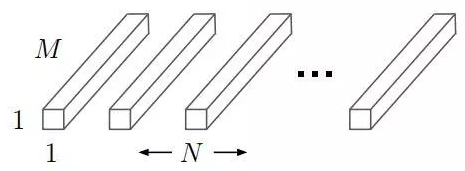
\includegraphics[width=0.5\linewidth]{Images/pointwise_1}
		\caption{Pointwise Conv,即$1\time 1$ 结构的普通卷积}
		\label{fig:pointwise1}
	\end{figure}

计算复杂度:
	\[
D_{K} \cdot D_{K} \cdot M \cdot N \cdot D_{F} \cdot D_{F}
\text{普通卷积}
\]	
\[
D_{K} \cdot D_{K} \cdot M \cdot D_{F} \cdot D_{F}+M \cdot N \cdot D_{F} \cdot D_{F}
\text{Depthwise + Pointwise Conv}
\]

\[
 \frac{D_{K} \cdot D_{K} \cdot M \cdot D_{F} \cdot D_{F}+M \cdot N \cdot D_{F} \cdot D_{F}}{D_{K} \cdot D_{K} \cdot M \cdot N \cdot D_{F} \cdot D_{F}} = \frac{1}{N}+\frac{1}{D_{K}^{2}} 
\]
\end{frame}

\begin{frame}{\titleprefix: MobileNet V2}
	\begin{figure}
		\centering
		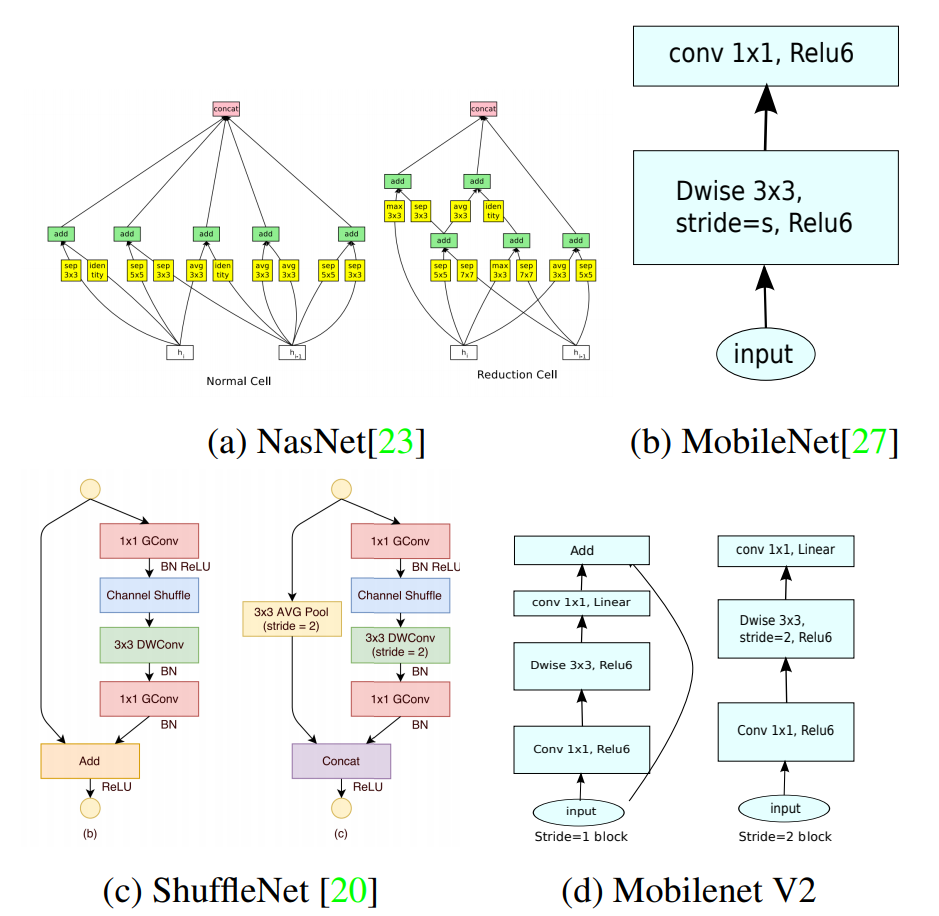
\includegraphics[width=0.6\linewidth]{Images/mobilenetv2}
		\caption{MobileNet V2与其它网络的对比}
		\label{fig:mobilenetv2}
	\end{figure}
	
\end{frame}

\begin{frame}{\titleprefix: MobileNet V3}
	\begin{figure}
		\centering
		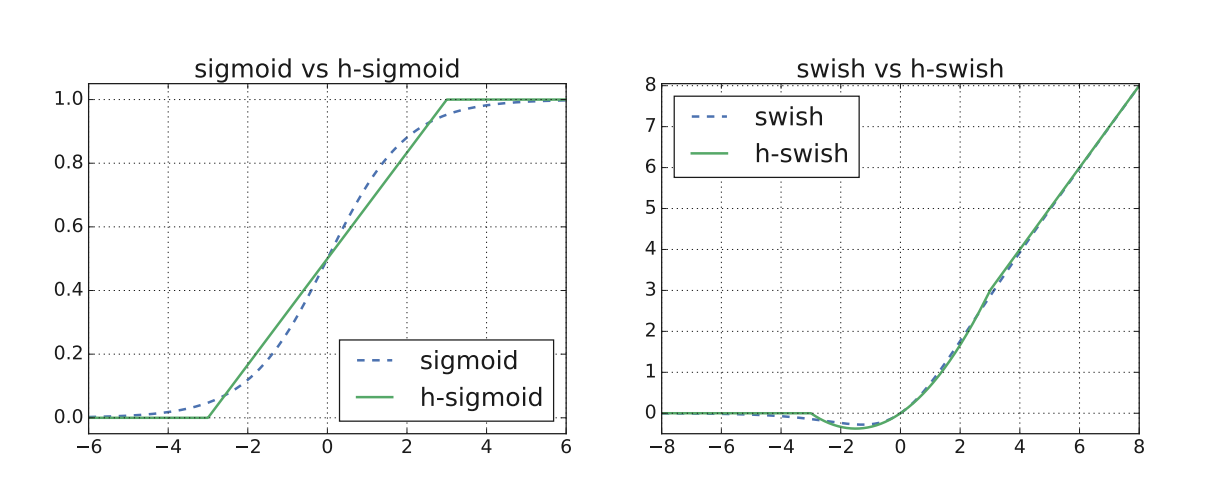
\includegraphics[width=0.9\linewidth]{Images/mobilenetv3}
		\caption{Sigmoid 和 Swish 的非线性形式及其hard近似}
		\label{fig:mobilenetv3}
	\end{figure}
	\[\text { swish } x=x \cdot \sigma(x)
	\hspace{1in}
	 \mathrm{h}-\text { swish }[x]=x
 \frac{\operatorname{Re} \mathrm{L} \mathrm{U} 6(x+3)}{6}\]
\end{frame}

\section{Discussions}

\begin{frame}{\titleprefix: 网络性能对比实验}
	\begin{figure}
		\centering
		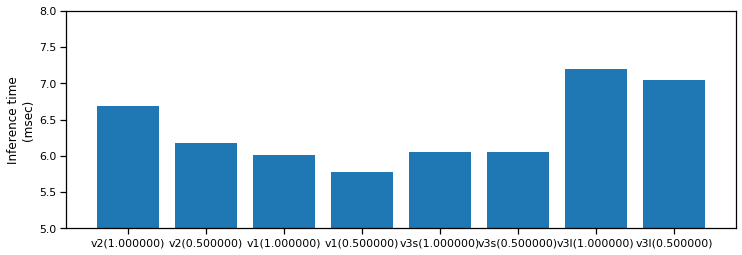
\includegraphics[width=0.7\linewidth]{Images/mobilenetcomp}
		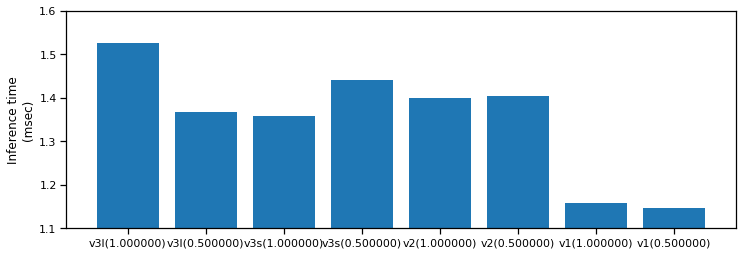
\includegraphics[width=0.7\linewidth]{Images/mobilenetcompgpu}
		\caption{各版本MobileNet在CPU和GPU上性能的表现}
		\label{fig:mobilenetcomp}
	\end{figure}

\end{frame}

\begin{frame}{\titleprefix: 如何改进现有网络}

		大家可以思考,根据今天讲到的网络特性,对于不同的实际使用环境,如何改进现有网络?

\end{frame}

\begin{frame}
	今天的内容结束了,谢谢大家。
\end{frame}